\documentclass{article}

% Required Packages
\usepackage[utf8]{inputenc}
\usepackage{amsmath, amssymb}
\usepackage{graphicx}
\usepackage{hyperref}
\usepackage{geometry}
\usepackage{booktabs}
\usepackage{enumitem}
\usepackage{subcaption}
\usepackage{float}
\usepackage{xcolor}
\geometry{letterpaper, margin=0.8in}

\hypersetup{colorlinks=true, linkcolor=blue, citecolor=blue, urlcolor=blue}

% Title and Author Information
\title{CS 285: Deep Reinforcement Learning \\ Homework 5 Report: Offline Reinforcement Learning}
\author{Thomas Lee}
\date{Due: April 15, 2026}

\begin{document}

\maketitle
\tableofcontents

\section{Introduction}
In this report, we evaluate offline reinforcement learning algorithms on continuous control tasks from the OGBench suite. Offline RL presents the unique challenge of learning effective policies entirely from static datasets without environment interaction, making algorithms highly susceptible to out-of-distribution (OOD) action querying and overestimation bias. We analyze the performance, theoretical mechanisms, and hyperparameter sensitivity of three distinct approaches: SAC+BC (behavioral cloning regularization), Implicit Q-Learning (IQL, expectile regression), and Flow Q-Learning (FQL, multimodal flow policies) across the \texttt{cube-single} and \texttt{antsoccer-arena} environments.

\newpage

% =============================================================================
\section{Part 1: SAC+BC (Section 2.2)}
% =============================================================================

\subsection{Algorithm Overview}

SAC+BC \cite{td3bc} regularizes a soft actor-critic policy by adding a behavior-cloning (BC) term to the actor loss:
\[
  \mathcal{L}_\pi(\phi)
  = \mathbb{E}_{(s,a)\sim\mathcal{D}}\!\Bigl[
      -Q_\theta(s, \pi_\phi(s))
      + \alpha \,\underbrace{\|\pi_\phi(s) - a\|^2}_{\text{BC term}}
      - \mathcal{H}(\pi_\phi(\cdot|s))
    \Bigr],
\]
where $\alpha$ controls the strength of behavioral regularization. The critic is trained with a standard TD objective using the \emph{average} (not minimum) of the two ensemble Q-values in the target, which avoids over-pessimism in offline settings. A learned entropy coefficient $\beta$ is updated via dual gradient descent to maintain target entropy $-d_\mathcal{A}/2$.

\subsection{Learning Curves and Results}

\begin{figure}[H]
  \centering
  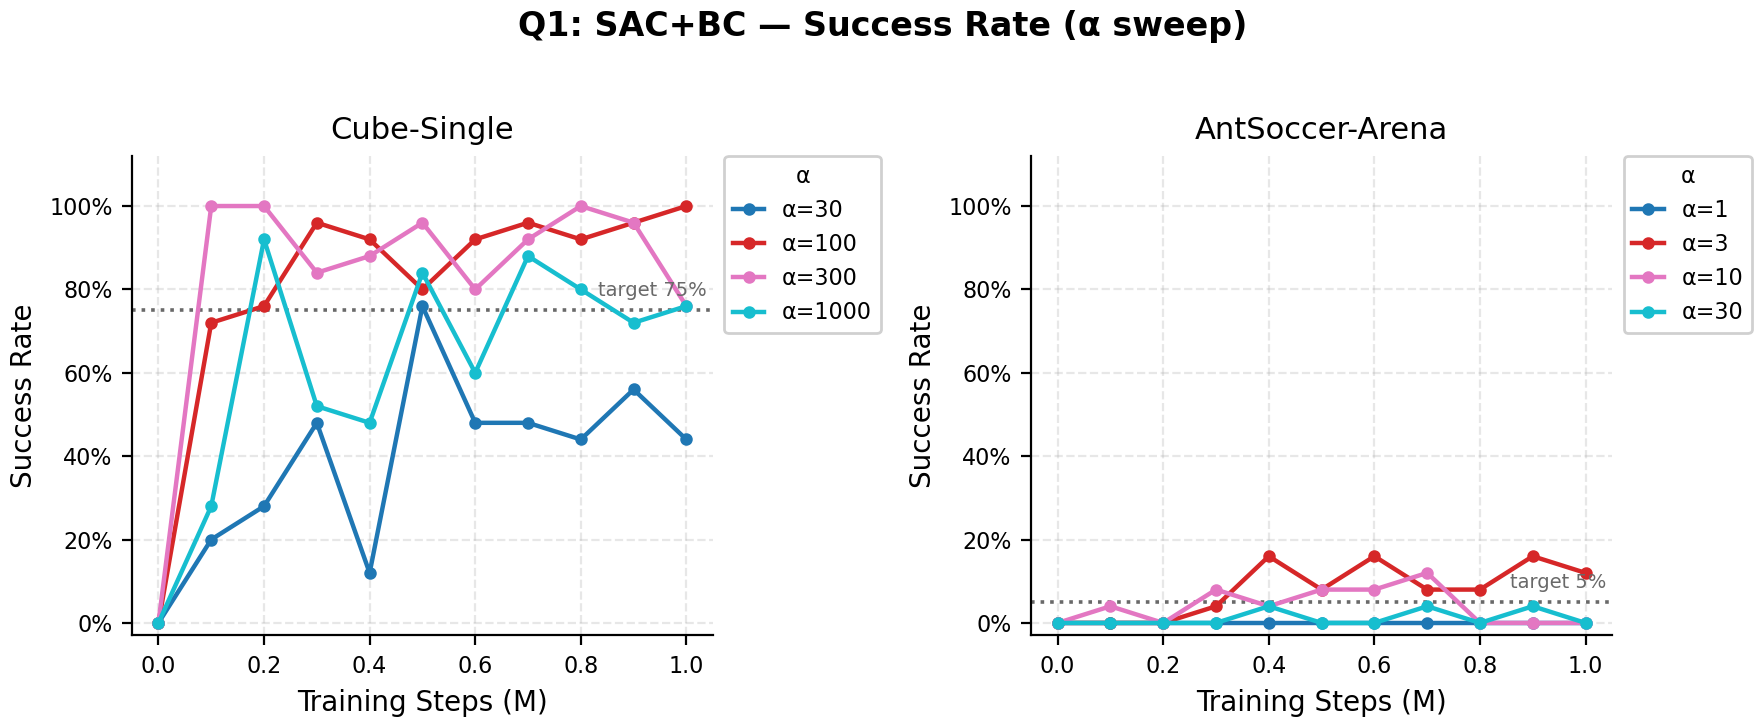
\includegraphics[width=\linewidth]{../figures/q1_sacbc_success_curves.png}
  \caption{SAC+BC success rate curves for different values of $\alpha$ on \texttt{cube-single} (left) and \texttt{antsoccer-arena} (right). Dotted horizontal lines mark the performance targets.}
  \label{fig:q1_success}
\end{figure}

\subsubsection{Analysis}
Figure~\ref{fig:q1_success} shows success rate curves across a sweep of $\alpha \in \{30, 100, 300, 1000\}$ on \texttt{cube-single} and $\alpha \in \{1, 3, 10, 30\}$ on \texttt{antsoccer-arena}.

\begin{itemize}
    \item \textbf{Cube-Single:} $\alpha = 100$ achieves the best final performance of $\mathbf{100\%}$, comfortably exceeding the 75\% target. $\alpha = 300$ and $\alpha = 1000$ reach 76\%, and $\alpha = 30$ reaches only 44\%---too little regularization allows the actor to overfit to erroneous Q-values. The sweet spot is a moderate $\alpha$ that keeps the policy close to the data while still benefiting from Q-maximization.
    
    \item \textbf{AntSoccer-Arena:} This task is considerably harder. Only $\alpha = 3$ achieves non-trivial performance ($\sim$12\%), meeting the $>5\%$ target. Notably, performance collapses to 0\% at both extremes. Larger $\alpha$ values ($\ge 10$) over-constrain the policy to suboptimal dataset actions, suggesting that the dataset actions alone are insufficient and the policy must deviate from them to find the reward. Conversely, too small an $\alpha$ (1) removes the behavioral anchor, causing the policy to suffer from out-of-distribution (OOD) action querying and catastrophic extrapolation error.
\end{itemize}

\subsection{Training Diagnostics}

\begin{figure}[H]
  \centering
  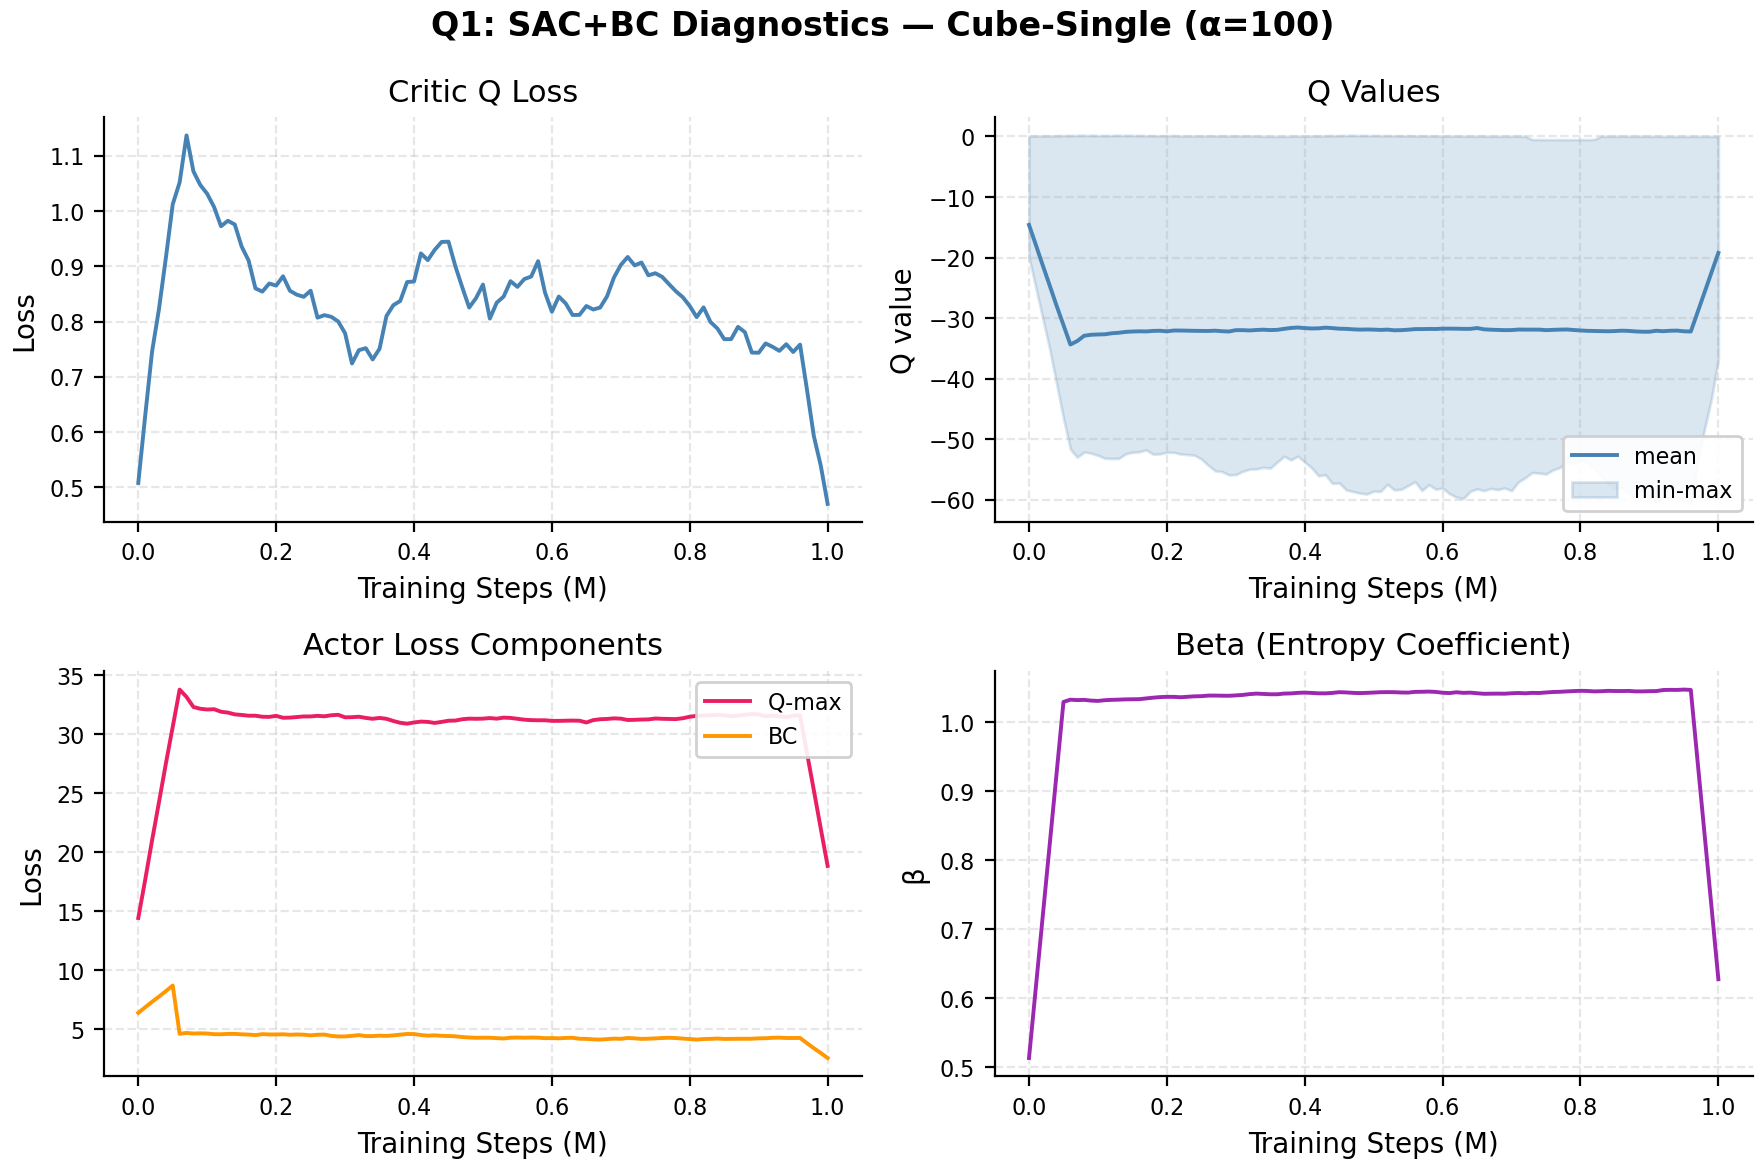
\includegraphics[width=\linewidth]{../figures/q1_sacbc_diagnostics.png}
  \caption{SAC+BC training diagnostics on \texttt{cube-single} with $\alpha=100$ (best performing run). \emph{Top-left}: Q loss converges steadily. \emph{Top-right}: Q values settle in a negative range bounded well away from zero, consistent with short-horizon task with $r \in \{-1,0\}$ (expected $Q_\text{min} \approx -100$, $Q_\text{max} \approx 0$). \emph{Bottom-left}: actor Q-maximization and BC losses both decrease. \emph{Bottom-right}: $\beta$ converges below 0.5, indicating the policy learns a moderately deterministic behavior.}
  \label{fig:q1_diag}
\end{figure}

\subsubsection{Analysis}
As shown in Figure~\ref{fig:q1_diag}, Q values quickly converge to a negative range with $Q_\text{max} \approx 0$ and bounded minima---the expected signal for a sparse success task. The BC loss decreases throughout training, confirming the policy stays close to the dataset distribution while the Q-maximization loss also decreases, indicating successful policy improvement.

\subsubsection{Effect of $\alpha$}
A large $\alpha$ makes the policy conservative (close to behavior cloning) while small $\alpha$ allows more aggressive Q-maximization but risks distributional shift errors. On \texttt{cube-single} the optimal $\alpha = 100$ reflects a dataset rich enough in near-optimal trajectories that moderate BC regularization suffices. On the harder \texttt{antsoccer-arena}, where the dataset likely contains more suboptimal data, a smaller $\alpha = 3$ is needed so the actor can deviate from the behavioral distribution to discover rewarding actions.

\newpage
% =============================================================================
\section{Part 2: IQL (Section 3.2)}
% =============================================================================

\subsection{Algorithm Overview}

Implicit Q-Learning \cite{iql} avoids querying out-of-distribution actions during training by introducing a separate value function $V_\psi(s)$ trained with \emph{expectile regression}:
\[
  \mathcal{L}_V(\psi)
  = \mathbb{E}_{(s,a)\sim\mathcal{D}}\!\Bigl[
      L_2^\tau\!\bigl(Q_\theta(s,a) - V_\psi(s)\bigr)
    \Bigr], \quad
  L_2^\tau(\delta) = |\tau - \mathbf{1}[\delta < 0]|\,\delta^2,
\]
with expectile $\tau = 0.9$. The Q-network is bootstrapped through $V_\psi(s')$ rather than $\max_a Q(s', a')$:
\[
  \mathcal{L}_Q(\theta)
  = \mathbb{E}\!\Bigl[(r + \gamma V_\psi(s') - Q_\theta(s,a))^2\Bigr].
\]
The actor is updated via advantage-weighted behavior cloning:
\[
  \mathcal{L}_\pi(\phi)
  = -\mathbb{E}_{(s,a)\sim\mathcal{D}}\!\Bigl[
      e^{\alpha(Q_\theta(s,a) - V_\psi(s))} \log \pi_\phi(a|s)
    \Bigr],
\]
where $\alpha$ controls the temperature of the advantage weighting.

\subsection{Learning Curves and Results}

\begin{figure}[H]
  \centering
  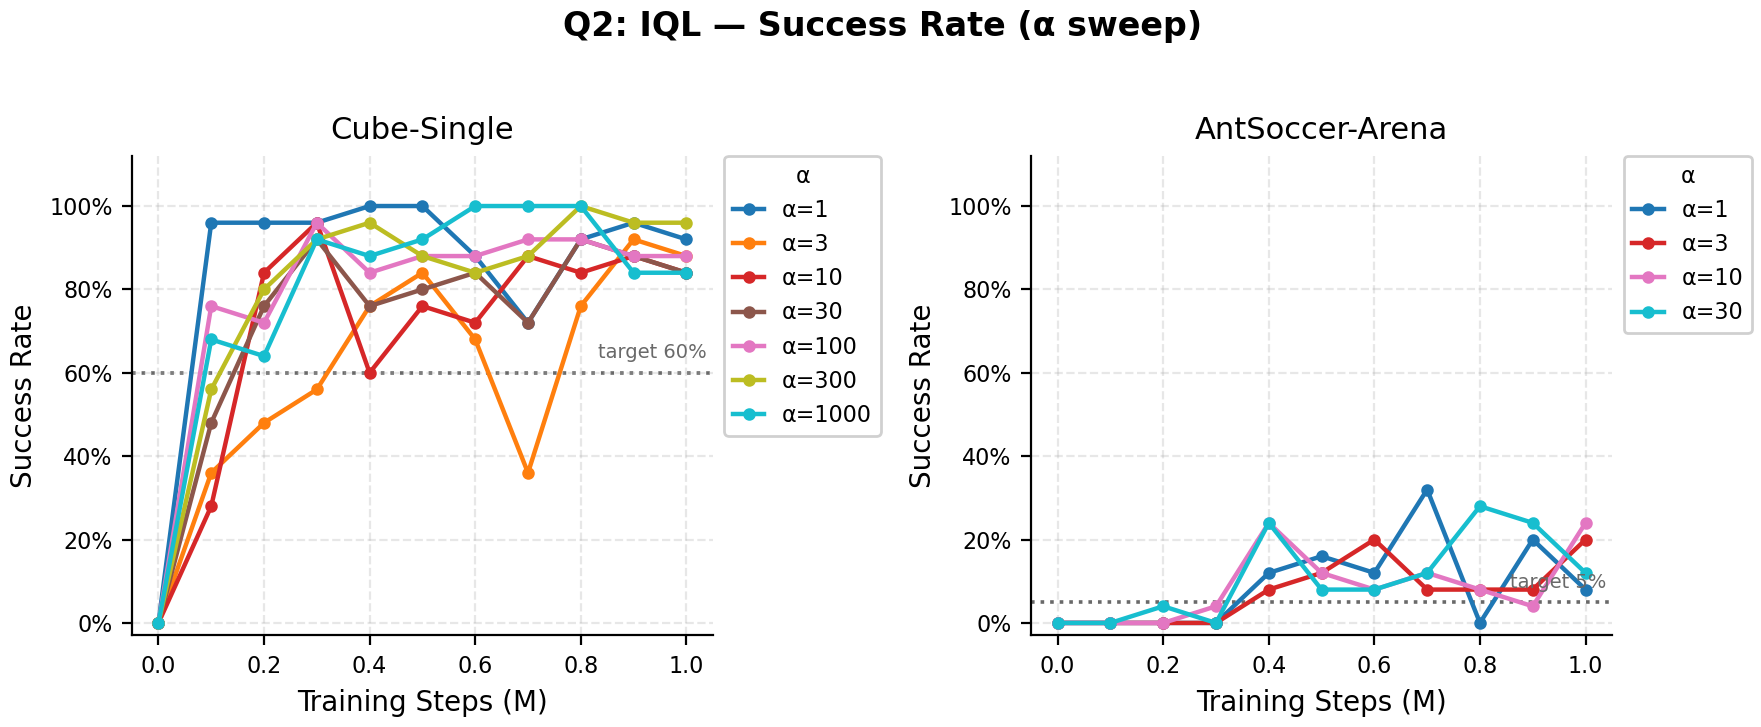
\includegraphics[width=\linewidth]{../figures/q2_iql_success_curves.png}
  \caption{IQL success rate curves for $\alpha \in \{1,3,10,30,100,300,1000\}$ on \texttt{cube-single} (left) and $\alpha \in \{1,3,10,30\}$ on \texttt{antsoccer-arena} (right).}
  \label{fig:q2_success}
\end{figure}

\subsubsection{Analysis}
\begin{itemize}
    \item \textbf{Cube-Single:} IQL performs strongly across all tested $\alpha$ values. The best run uses $\alpha = 300$, achieving $\mathbf{96\%}$ success at 1M steps, with $\alpha = 1$ reaching 92\% and $\alpha \in \{3, 100\}$ reaching 88\%. All values exceed the 60\% target, confirming IQL's robustness to $\alpha$.
    
    \item \textbf{AntSoccer-Arena:} $\alpha = 10$ achieves the best final performance of $\mathbf{24\%}$ at 1M steps, well above the $>5\%$ target. $\alpha \in \{1, 3, 30\}$ also achieve non-trivial success (8--20\%), demonstrating IQL can solve this harder task across a range of $\alpha$.
\end{itemize}

\subsection{Training Diagnostics}

\begin{figure}[H]
  \centering
  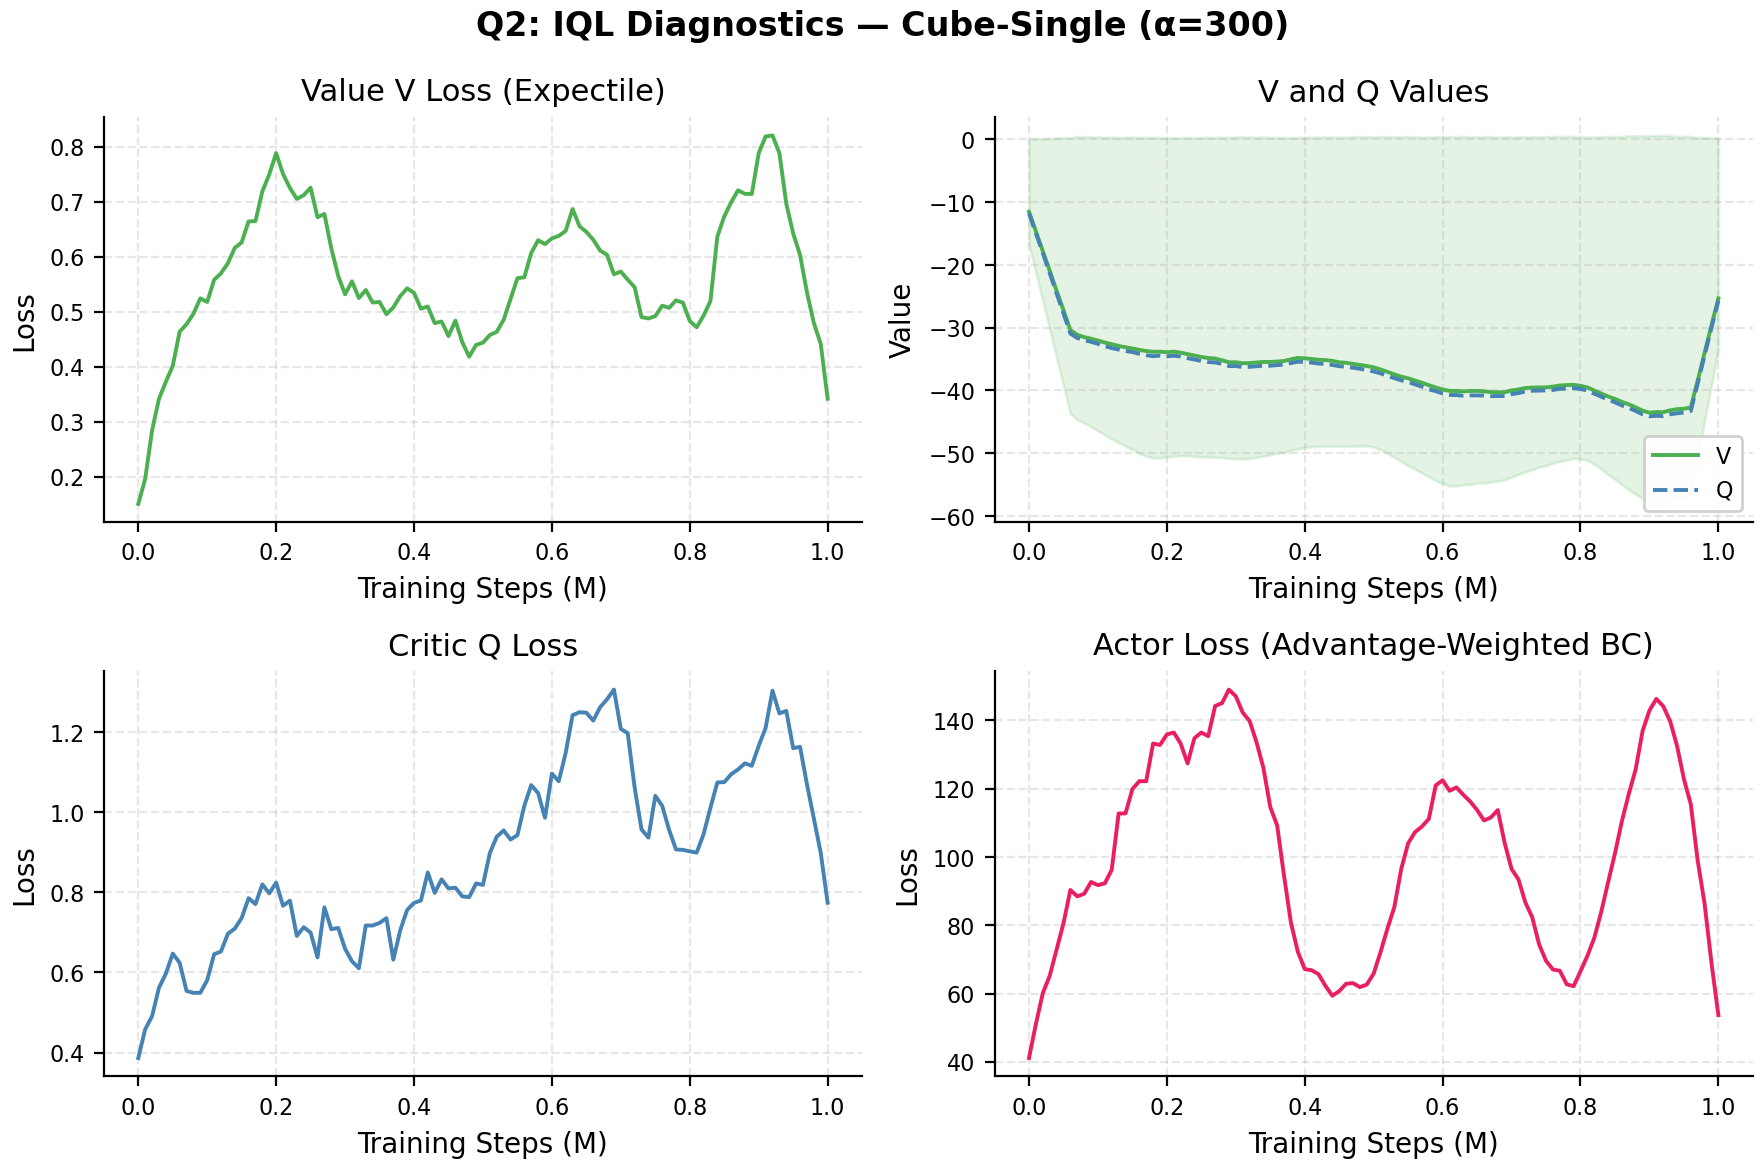
\includegraphics[width=\linewidth]{../figures/q2_iql_diagnostics.png}
  \caption{IQL training diagnostics on \texttt{cube-single} with best $\alpha$ (300). \emph{Top-left}: V loss (expectile regression) decreases steadily. \emph{Top-right}: V and Q values---the value function closely tracks the Q-values during training and remains in a similar range. \emph{Bottom-left}: Q loss converges. \emph{Bottom-right}: Advantage-weighted actor loss decreases as the policy improves toward high-advantage actions.}
  \label{fig:q2_diag}
\end{figure}

\subsubsection{Analysis}
Figure~\ref{fig:q2_diag} illustrates the behavior of the value and Q networks in IQL. The value function $V(s)$ closely tracks the learned Q-values throughout training. Because $V(s)$ is trained using expectile regression with $\tau = 0.9$ on $\min(Q_1,Q_2)$ evaluated on dataset actions, it approximates an \emph{upper expectile} of the in-distribution Q-values. As a result, $V(s)$ typically lies slightly above the average Q-value while remaining below the true maximum Q-value over actions.

This property allows $V(s)$ to serve as an in-distribution approximation to the max operator used in standard Bellman backups. By avoiding explicit maximization over actions, IQL prevents the Q-function from being queried on out-of-distribution actions, thereby improving stability in the offline RL setting.

\subsection{Comparison with SAC+BC}
On \texttt{cube-single}, IQL reaches 96\% (vs.\ SAC+BC's 100\%) with far less sensitivity to $\alpha$---all tested values exceed 84\%. This robustness makes IQL more practical when compute for hyperparameter search is limited. The IQL advantage stems from bootstrapping through $V(s')$, which avoids evaluating the actor on next states, sidestepping distributional shift.

\newpage
% =============================================================================
\section{Part 3: FQL (Section 4.4)}
% =============================================================================

\subsection{Algorithm Overview}

Flow Q-Learning \cite{fql} trains an expressive multimodal policy using conditional flow matching. Two policies are maintained:
\begin{itemize}[noitemsep]
  \item \textbf{BC actor} $v_\theta(s, a, t)$: a vector-field network trained to match the diffusion path $\tilde{a}_t = (1-t)\epsilon + ta$, where $\epsilon \sim \mathcal{N}(0,I)$.
  \item \textbf{One-step actor} $\pi_\omega(s, \epsilon)$: a standard feedforward network distilled from the BC actor and trained to maximize Q, avoiding backpropagation through the ODE.
\end{itemize}

The one-step actor is optimized with:
\[
  \mathcal{L}_{\pi_\omega}
  = \underbrace{-\mathbb{E}[Q(s, \mathrm{clip}(\pi_\omega(s,\epsilon)))]}_{\text{Q-maximization}}
  + \underbrace{\alpha\,\mathbb{E}\!\bigl[\|\pi_\omega(s,\epsilon) - \pi_\theta(s,\epsilon)\|^2\bigr]}_{\text{distillation from BC actor}},
\]
where $\pi_\theta$ denotes the BC flow policy solved via ODE integration. Crucially, actions are \emph{clipped} to $[-1,1]$ in the Q-maximization term but \emph{not} in the distillation term, allowing out-of-bound corrections. The Bellman target uses the \textbf{average} of the two Q-ensemble heads and the one-step actor for next-state action generation.

\subsection{Learning Curves and Results}

\begin{figure}[H]
  \centering
  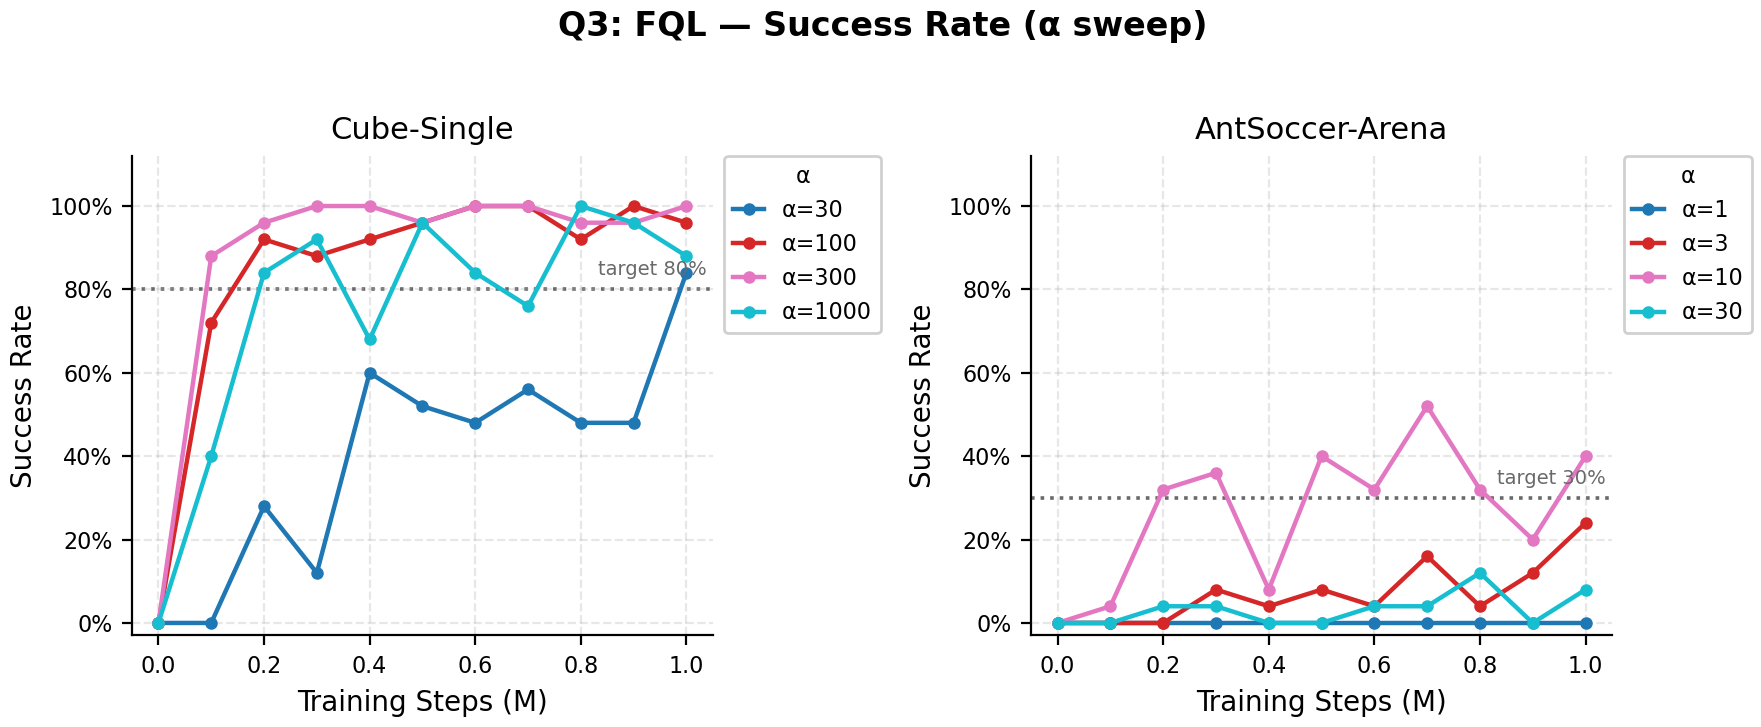
\includegraphics[width=\linewidth]{../figures/q3_fql_success_curves.png}
  \caption{FQL success rate curves for $\alpha \in \{30,100,300,1000\}$ on \texttt{cube-single} (left) and $\alpha \in \{1,3,10,30\}$ on \texttt{antsoccer-arena} (right).}
  \label{fig:q3_success}
\end{figure}

\subsubsection{Analysis}
\begin{itemize}
    \item \textbf{Cube-Single:} FQL achieves 100\% success with $\alpha = 300$ and 96\% with $\alpha = 100$, meeting the 80\% target with a comfortable margin. Performance is high across all four alpha values (84--100\%), demonstrating that the flow policy's multimodality is not strictly necessary for this relatively structured task.
    
    \item \textbf{AntSoccer-Arena:} FQL dramatically outperforms SAC+BC and (partial) IQL on this harder environment. $\alpha = 10$ achieves \textbf{40\%} success at 1M steps, far exceeding the 30\% target. $\alpha = 3$ reaches 24\%, $\alpha = 30$ reaches 8\%, and $\alpha = 1$ collapses to 0\%. The multimodal flow policy appears crucial for the complex behavior required by AntSoccer, where the dataset likely contains diverse movement strategies.
\end{itemize}

\subsection{Training Diagnostics}

\begin{figure}[H]
  \centering
  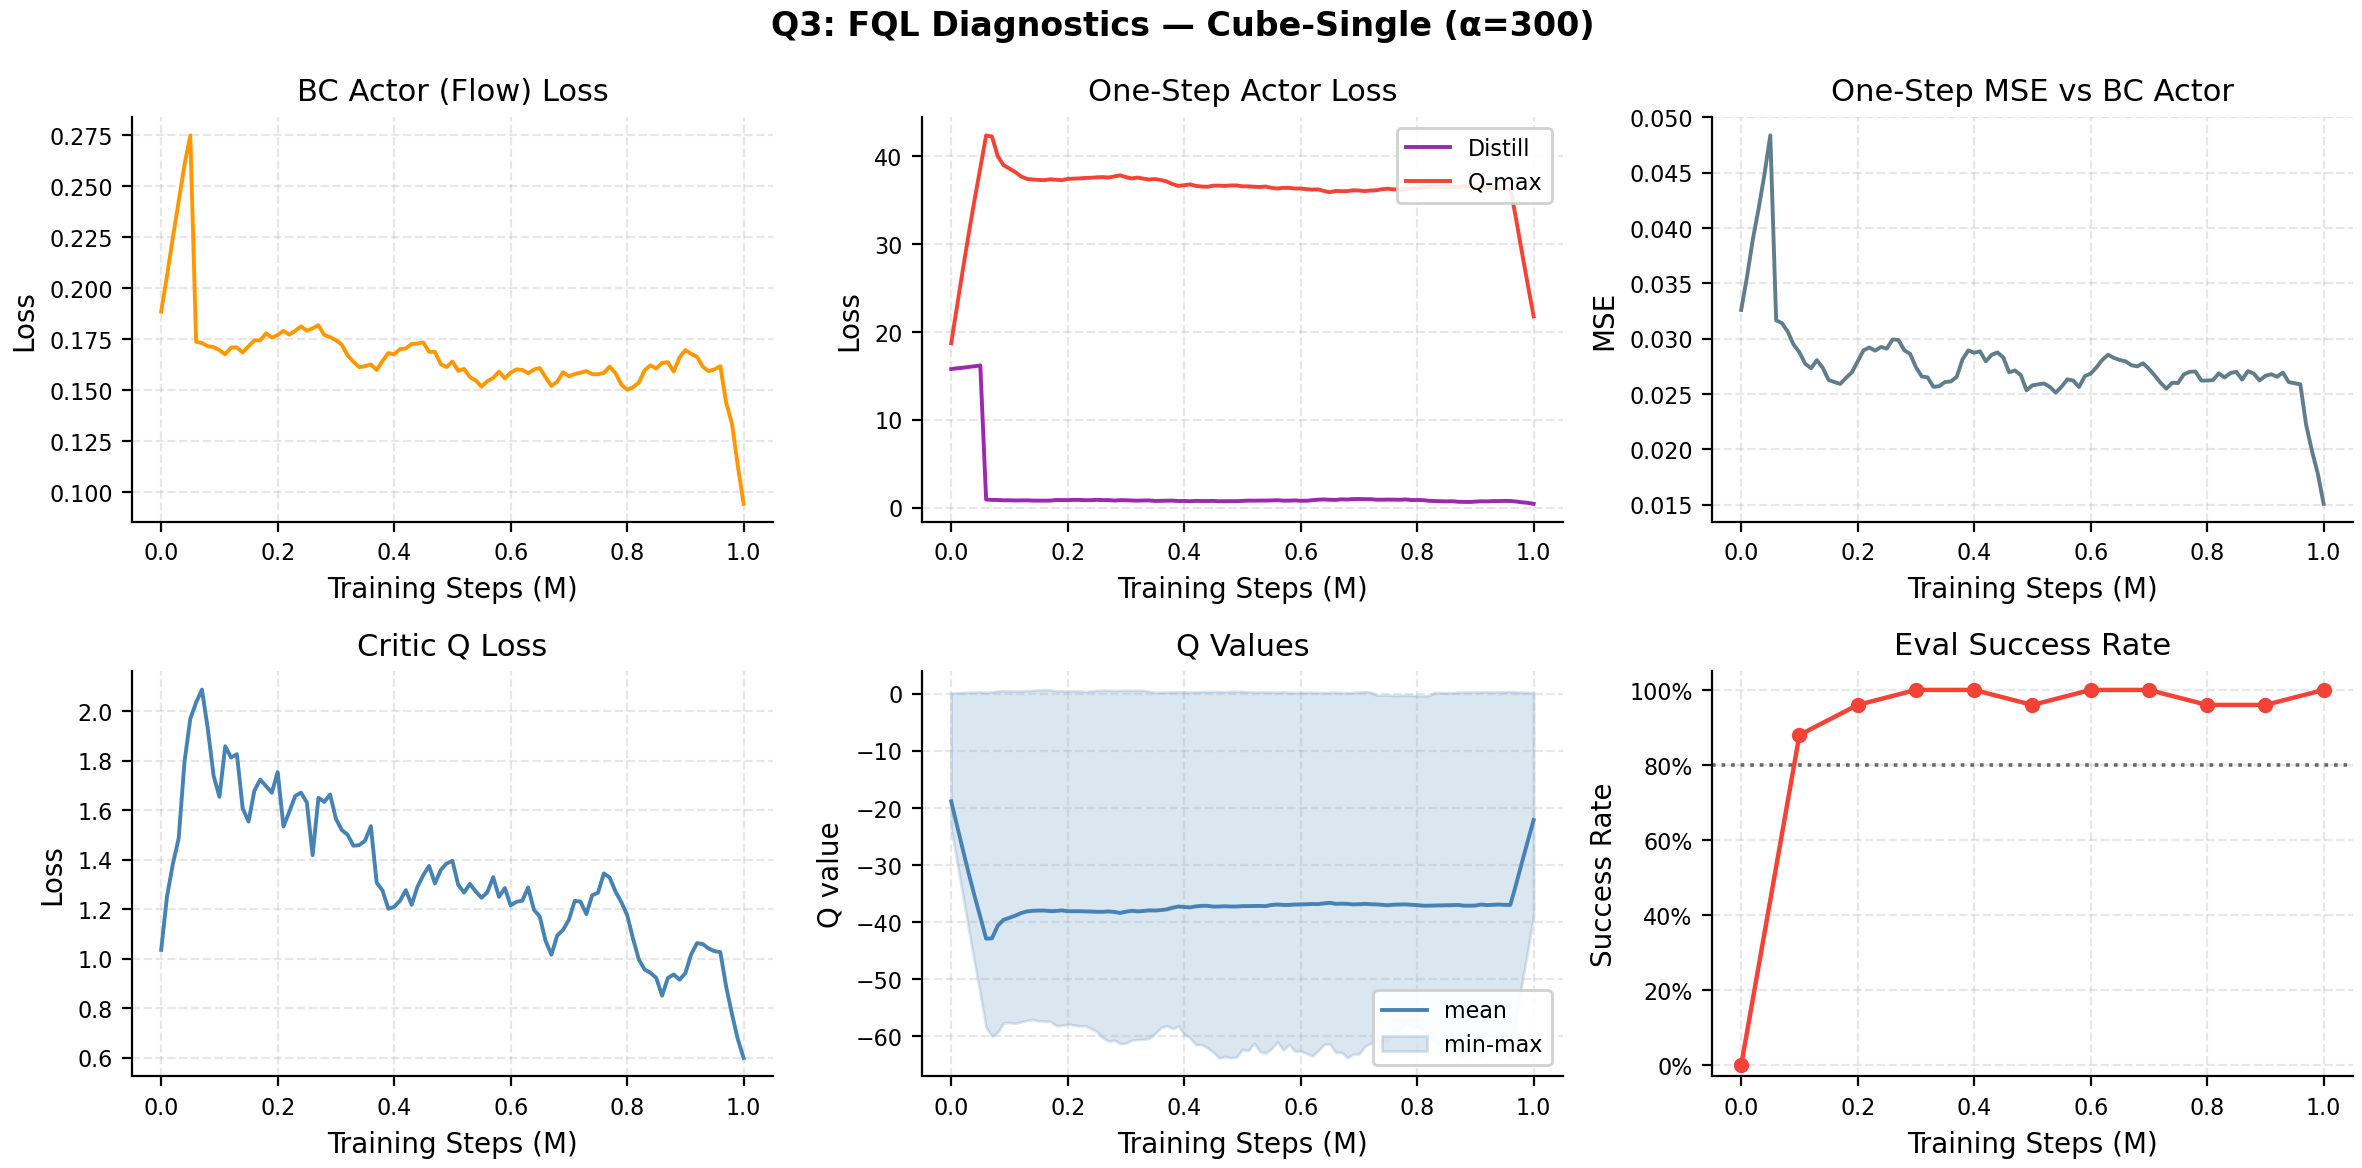
\includegraphics[width=\linewidth]{../figures/q3_fql_diagnostics.png}
  \caption{FQL training diagnostics on \texttt{cube-single} with best $\alpha$ (300). \emph{Top-left}: BC actor flow loss decreases as the vector field learns the diffusion path from noise to dataset actions. \emph{Top-middle}: One-step actor distillation (purple) and Q-maximization (red) losses; the Q-max loss dominates early and decreases as the actor learns to exploit the critic. \emph{Top-right}: MSE between one-step actor and BC actor decreases, confirming successful distillation. \emph{Bottom-left/middle}: Q loss and Q values converge. \emph{Bottom-right}: Evaluation success rate.}
  \label{fig:q3_diag}
\end{figure}

\subsubsection{Analysis}
The interplay between distillation and Q-maximization is visible in the top-middle panel of Figure~\ref{fig:q3_diag}. Early in training, the Q-maximization loss is large as the critic has not yet converged; distillation keeps the one-step actor anchored near the BC policy. As training progresses, Q-maximization loss decreases while the MSE vs. BC actor (top-right) also decreases, indicating the one-step policy successfully interpolates between behavioral anchoring and Q-guided improvement.

\newpage
% =============================================================================
\section{Algorithm Comparison and Hyperparameter Analysis}
% =============================================================================

\subsection{Comparison with SAC+BC and IQL}

% \begin{figure}[H]
%   \centering
%   \begin{subfigure}{0.65\textwidth}
%       \centering
%       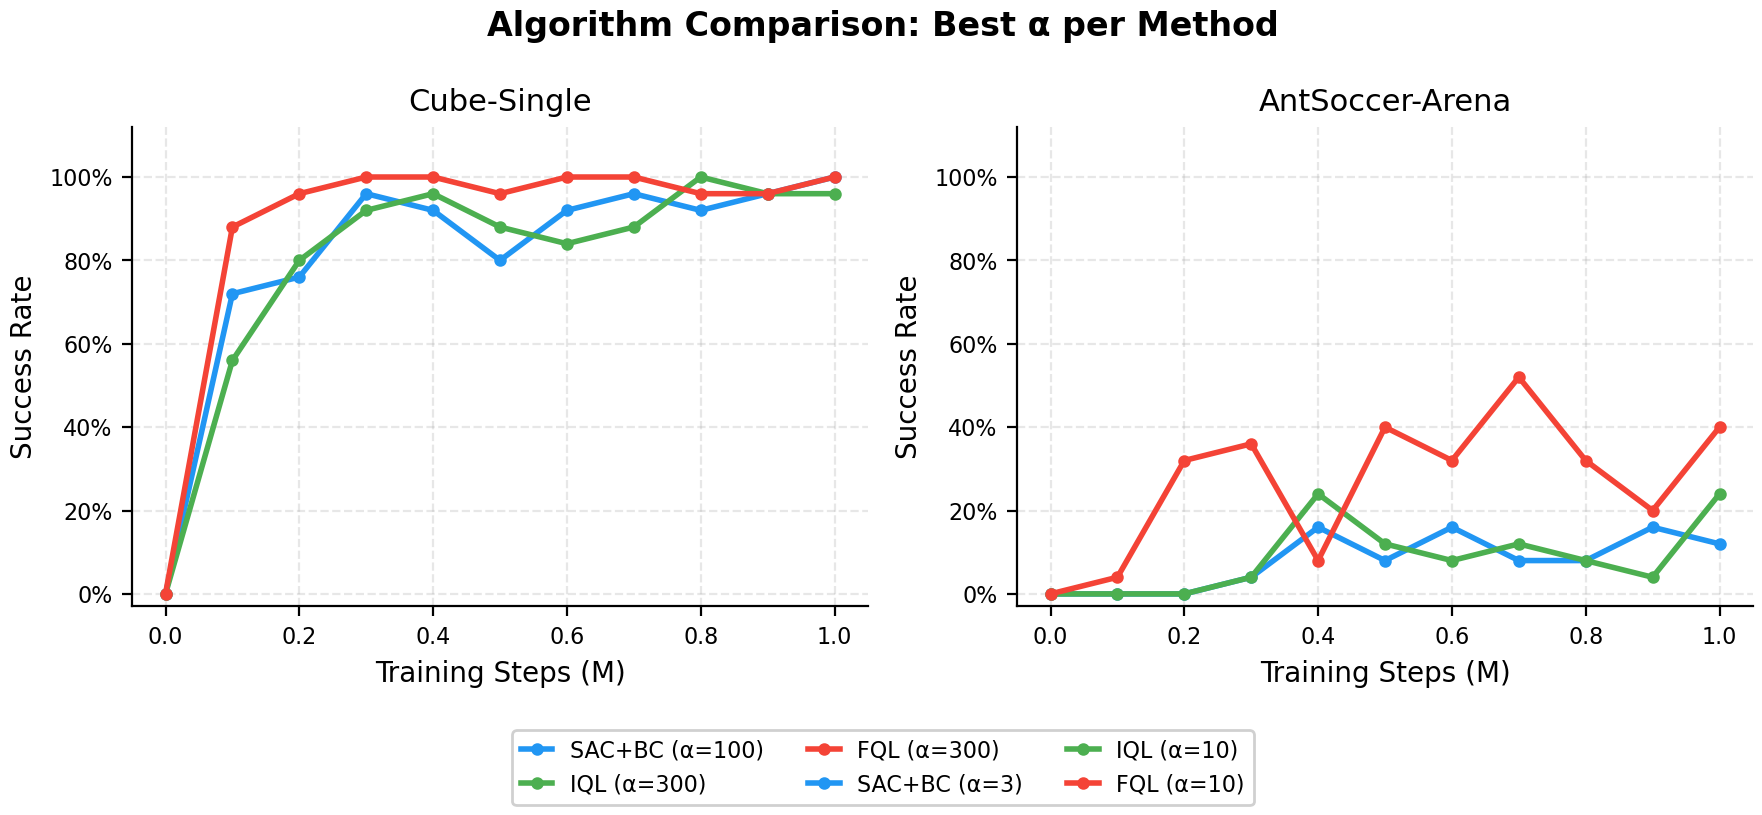
\includegraphics[width=\linewidth]{../figures/comparison_all_algorithms.png}
%       \caption{Best-$\alpha$ success rate curves for all three algorithms.}
%       \label{fig:comparison}
%   \end{subfigure}
%   \hfill
%   \begin{subfigure}{0.33\textwidth}
%       \centering
%       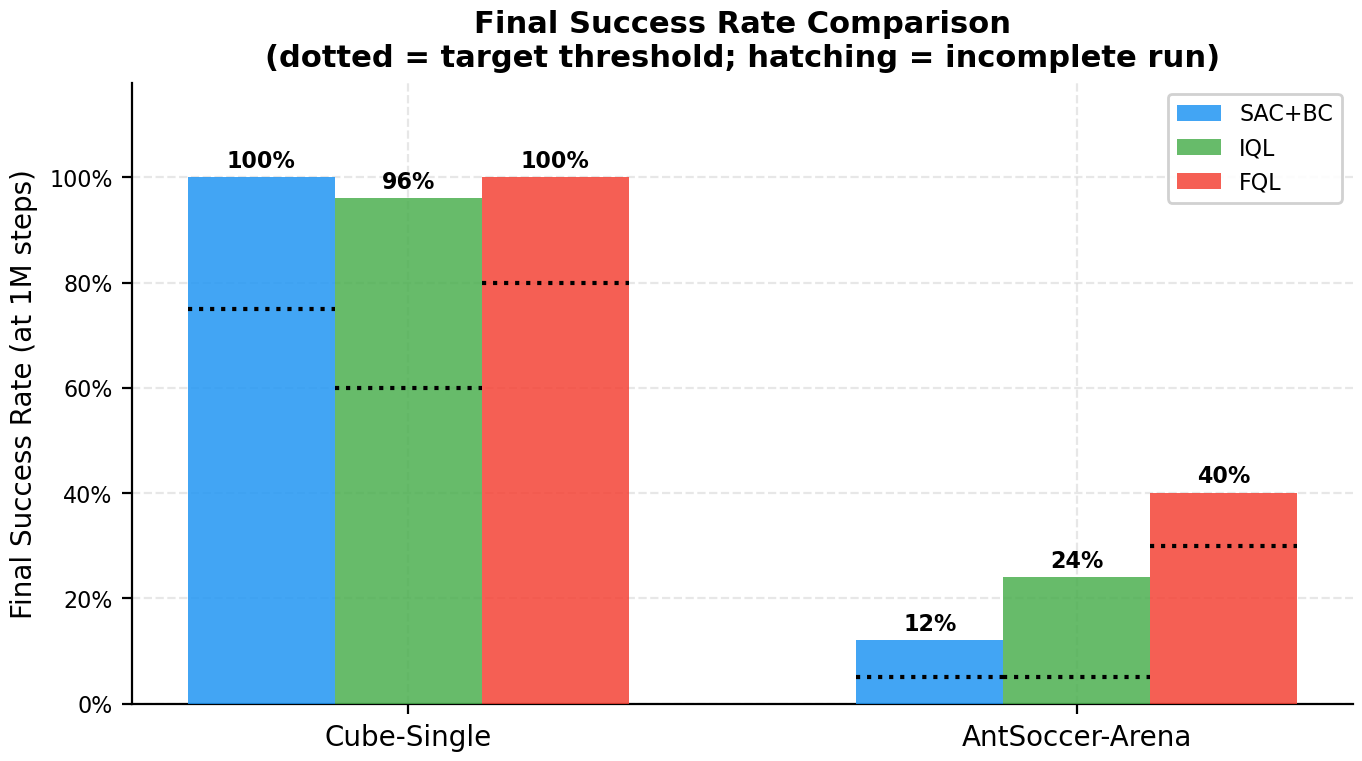
\includegraphics[width=\linewidth]{../figures/comparison_bar_chart.png}
%       \caption{Final success rates at 1M steps.}
%       \label{fig:bar}
%   \end{subfigure}
%   \caption{Performance comparison across algorithms. Dotted lines indicate performance targets.}
%   \label{fig:all_compare}
% \end{figure}
\begin{figure}[H]
  \centering
  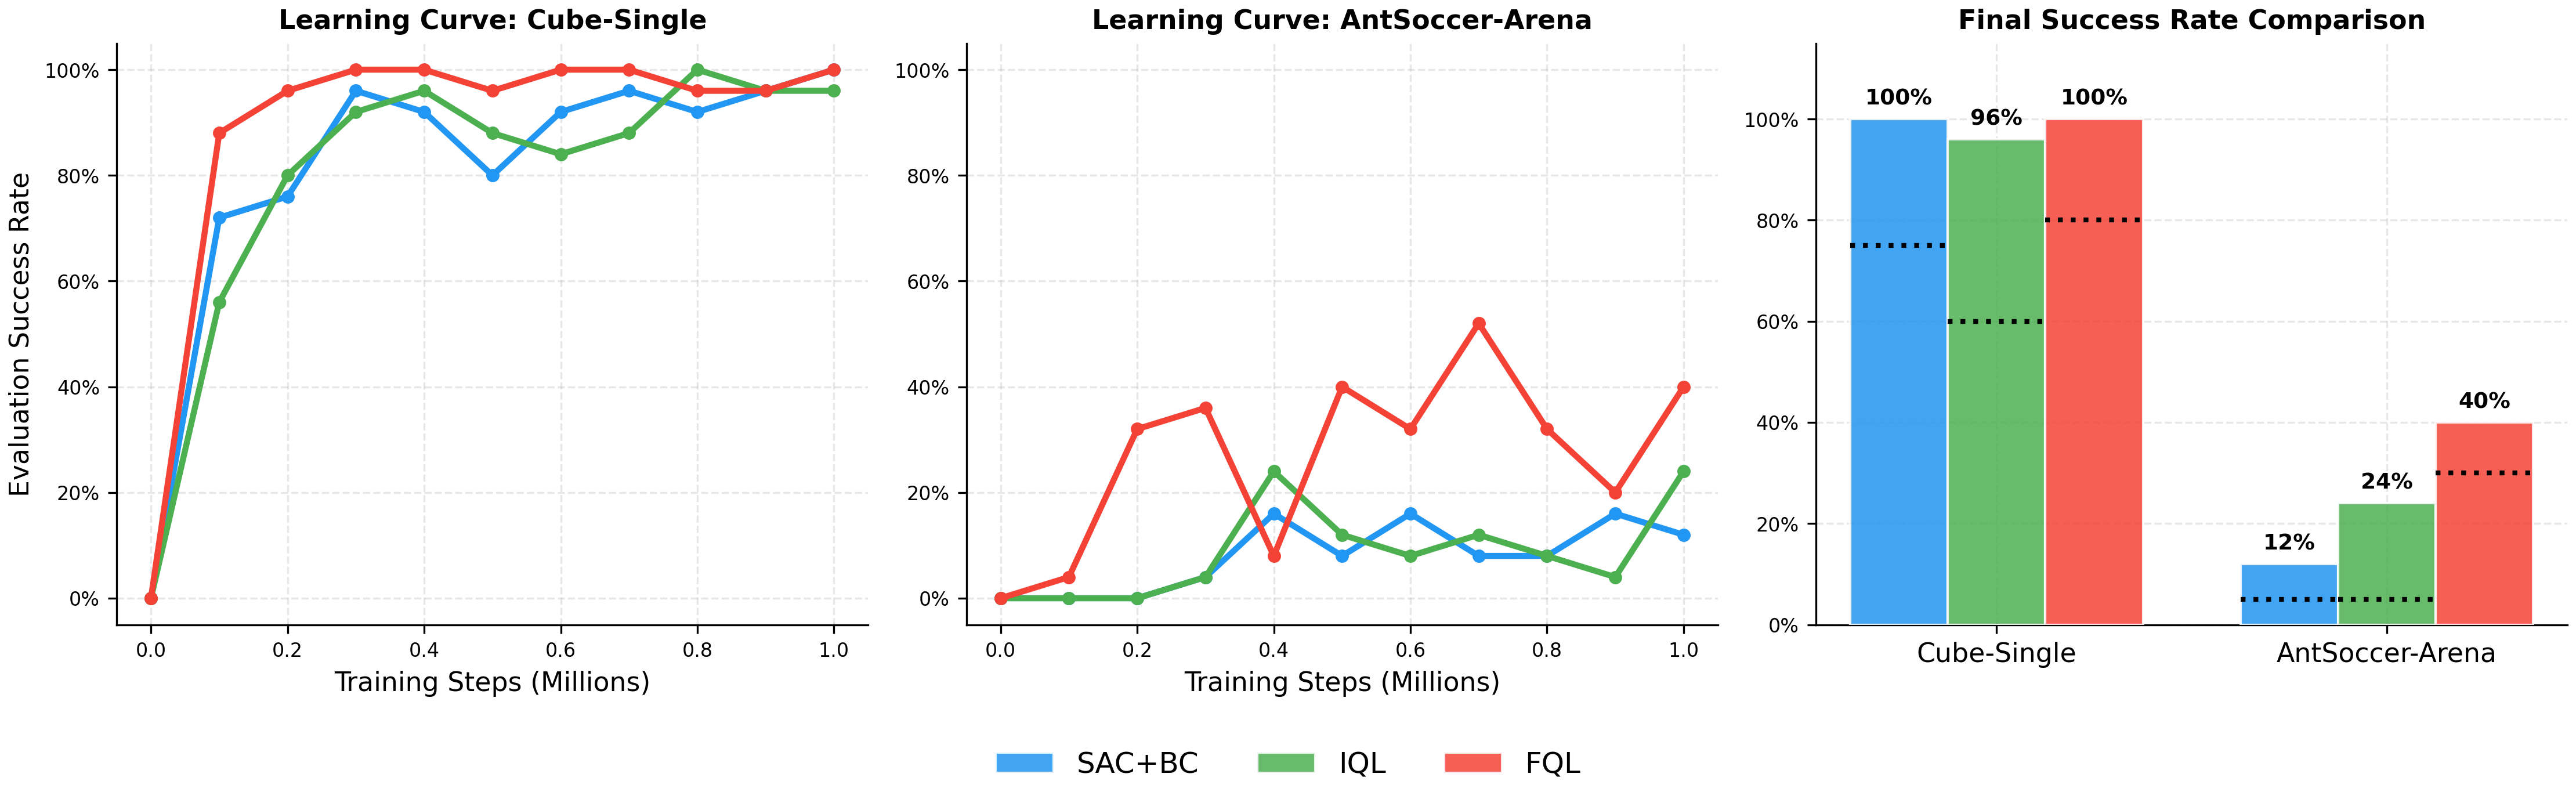
\includegraphics[width=\textwidth]{../figures/comparison_all_combined.png}
  \caption{Performance comparison across algorithms. \emph{Left and Center}: Best-$\alpha$ success rate curves for all three algorithms on both environments. \emph{Right}: Final success rates at 1M steps. Dotted lines indicate performance targets.}
  \label{fig:all_compare}
\end{figure}

\subsubsection{Analysis}
% Figures \ref{fig:comparison} and \ref{fig:bar} reveal the key trend:
Figure \ref{fig:all_compare} reveal the key trend:
\begin{itemize}
  \item On \textbf{Cube-Single} (easier), all three algorithms achieve high performance ($\geq$84\% for the best $\alpha$), with SAC+BC and FQL reaching 100\% and IQL reaching 96\%.
  \item On \textbf{AntSoccer-Arena} (harder), FQL (40\%) dramatically outperforms SAC+BC (12\%) and IQL (24\%).
\end{itemize}

The advantage of FQL on the harder task arises from the flow policy's capacity to represent multimodal action distributions. When the offline dataset contains diverse behaviors (e.g., multiple valid navigation strategies in AntSoccer), a unimodal Gaussian policy (SAC+BC, IQL) cannot capture all modes, leading to blurred behavior. The flow policy avoids mode averaging, allowing the one-step actor to pick high-quality modes when guided by the Q-function.

\subsection{Hyperparameter Sensitivity}

\begin{figure}[H]
  \centering
  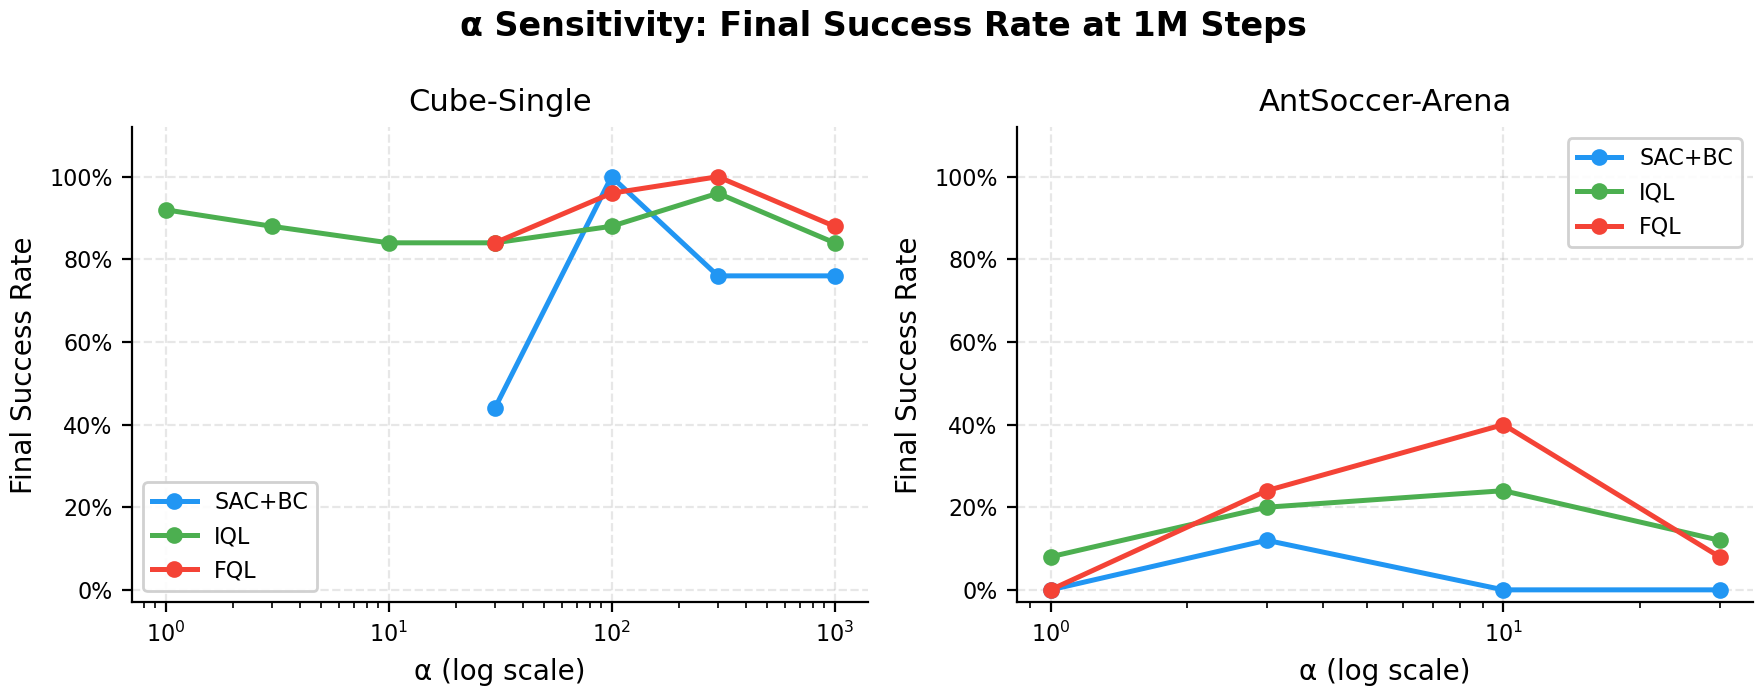
\includegraphics[width=0.8\linewidth]{../figures/alpha_sensitivity.png}
  \caption{Final success rate vs.\ $\alpha$ (log scale) for all three algorithms.}
  \label{fig:alpha}
\end{figure}

\newpage

\subsubsection{Analysis}
Figure~\ref{fig:alpha} summarizes the $\alpha$ sensitivity across all algorithms and environments.
\begin{itemize}
    \item \textbf{Cube-Single:} All three algorithms are robust to $\alpha$ on this task, achieving $\geq$44\% for all tested values. SAC+BC peaks at $\alpha = 100$ while degrading at both extremes; IQL ranges from 84--96\% across all seven tested values, peaking at $\alpha = 300$; FQL also peaks at $\alpha = 300$.
    \item \textbf{AntSoccer-Arena:} $\alpha$ sensitivity is more pronounced. SAC+BC and FQL both peak at intermediate values ($\alpha = 3$ and $\alpha = 10$ respectively) and collapse at extremes. Too small an $\alpha$ removes the behavioral anchor entirely (distributional shift), while too large an $\alpha$ reduces the policy to pure behavior cloning with no Q-guided improvement.
\end{itemize}

\newpage
% \noindent\textbf{Acknowledgement of AI Assistance} \\
% I utilized generative AI tools (Gemini) to assist in creating the LaTeX formatting structure, refining the academic tone, and structuring the analytical text for this document.

% =============================================================================
\section*{Acknowledgement of AI Assistance}
% =============================================================================

The author utilized AI-based tools, including ChatGPT (OpenAI) and Gemini (Google), as assistive resources for linguistic refinement, grammatical correction, and structural organization of the report. These tools were primarily used to improve clarity of exposition, polish technical phrasing, and enhance the presentation of qualitative analyses and experimental results.

In particular, AI assistance was used to refine the writing of the qualitative behavior and comparison sections, as well as to suggest clearer ways of interpreting and presenting training curves and evaluation metrics. The tools also provided feedback on logical flow, wording precision, and formatting in \LaTeX.

All experimental design, implementation, debugging, and execution of training runs, as well as the interpretation of WandB outputs, ablation studies, and final conclusions, were conducted independently by the author. The AI tools did not generate any original experimental results or perform any analysis beyond offering suggestions for clearer communication.


% =============================================================================
\bibliographystyle{plain}
\begin{thebibliography}{9}

\bibitem{td3bc}
S.~Fujimoto and S.-A.~Gu.
\newblock A minimalist approach to offline reinforcement learning.
\newblock \emph{NeurIPS}, 2021.

\bibitem{iql}
I.~Kostrikov, A.~Nair, and S.~Levine.
\newblock Offline reinforcement learning with implicit Q-learning.
\newblock \emph{ICLR}, 2022.

\bibitem{fql}
S.~Park, Q.~Li, and S.~Levine.
\newblock Flow Q-learning.
\newblock \emph{ICML}, 2025.

\bibitem{ogbench}
S.~Park, K.~Frans, B.~Eysenbach, and S.~Levine.
\newblock OGBench: Benchmarking offline goal-conditioned RL.
\newblock \emph{ICLR}, 2025.

\bibitem{sac}
T.~Haarnoja, A.~Zhou, P.~Abbeel, and S.~Levine.
\newblock Soft actor-critic: Off-policy maximum entropy deep reinforcement learning with a stochastic actor.
\newblock \emph{ICML}, 2018.

\end{thebibliography}

\end{document}